
\documentclass[a4paper]{article}
\usepackage{fancyhdr}
\usepackage[top=3cm, bottom=2cm, left=2cm, right=4cm]{geometry}
\usepackage[english]{babel}
\usepackage[utf8]{inputenc}
\usepackage{cite} % Bibtex package
\usepackage{amsmath}
\usepackage{amssymb}
\usepackage{amsfonts}
\usepackage{graphicx}
\usepackage{float}
\usepackage{caption}
\usepackage{subcaption}
\usepackage{amsthm}
\newtheorem{thm}{Sætning}
\newtheorem{dfn}{Definition}
\usepackage{lmodern}
\graphicspath{{./pictures/}}
%\usepackage{textpos}
\usepackage{color}
\usepackage{xcolor}
\usepackage{listingsutf8}
\usepackage{courier}
\usepackage{epstopdf}
\usepackage{fixltx2e}

%\epstopdfsetup{update,prepend,verbose,suffix=-generated} % use suffix because you don't want to accidentally overwrite a file that might have been a pdf source. The epstopdf package manual has more on that.

 
 \usepackage{hyperref}

%palatino
% Palatino for rm and math | Helvetica for ss | Courier for tt
\usepackage{mathpazo} % math & rm
\usepackage{mathrsfs}
\linespread{1.05}        % Palatino needs more leading (space between lines)
%\usepackage[scaled]{helvet} % ss
%\usepackage{courier} % tt
%\normalfont
%\usepackage[T1]{fontenc}
 \usepackage{bm}
\definecolor{javared}{rgb}{0.6,0,0} % for strings
\definecolor{javagreen}{rgb}{0.25,0.5,0.35} % comments
\definecolor{javapurple}{rgb}{0.5,0,0.35} % keywords
\definecolor{javadocblue}{rgb}{0.25,0.35,0.75} % javadoc
\definecolor{mauve}{rgb}{0.6,0,0}
%\definecolor{box}{rgb}{0.98,0.98,0.98} % box

%TESTTESTTEST

%setup listings
\lstset{language=C,
  extendedchars=true,
  %language=Octave,                % the language of the code
  basicstyle=\ttfamily\footnotesize,% the size of the fonts that are used for the code
  numbers=left,                   % where to put the line-numbers
  numberstyle=\tiny\color{gray},  % the style that is used for the line-numbers
  stepnumber=2,                   % the step between two line-numbers. If it's 1, each line 
                                  % will be numbered
  numbersep=5pt,                  % how far the line-numbers are from the code
  backgroundcolor=\color{white},      % choose the background color. You must add \usepackage{color}
  showspaces=false,               % show spaces adding particular underscores
  showstringspaces=false,         % underline spaces within strings
  showtabs=false,                 % show tabs within strings adding particular underscores
  frame=single,                   % adds a frame around the code
  rulecolor=\color{black},        % if not set, the frame-color may be changed on line-breaks within not-black text (e.g. comments (green here))
  tabsize=4,                      % sets default tabsize to 2 spaces
  captionpos=b,                   % sets the caption-position to bottom
  breaklines=true,                % sets automatic line breaking
  breakatwhitespace=false,        % sets if automatic breaks should only happen at whitespace
  title=\lstname,                   % show the filename of files included with \lstinputlisting;
                                  % also try caption instead of title
  keywordstyle=\color{blue},          % keyword style
  commentstyle=\color{javagreen},       % comment style
  stringstyle=\color{javared},         % string literal style
  escapeinside={\%*}{*)},            % if you want to add LaTeX within your code
  morekeywords={*,...},              % if you want to add more keywords to the set
  deletekeywords={...}              % if you want to delete keywords from the given language
}
\lstset{literate=%
{æ}{{\ae}}1
{å}{{\aa}}1
{ø}{{\o}}1
{Æ}{{\AE}}1
{Å}{{\AA}}1
{Ø}{{\O}}1
{°}{{${}^o$}}1
{I̅}{{$\overline{\mbox{I}}$}}1
{X̅}{{$\overline{\mbox{X}}$}}1
{V̅}{{$\overline{\mbox{V}}$}}1
{L̅}{{$\overline{\mbox{L}}$}}1
{D̅}{{$\overline{\mbox{D}}$}}1
{C̅}{{$\overline{\mbox{C}}$}}1
{M̅}{{$\overline{\mbox{M}}$}}1
{M̅}{{$\overline{\mbox{M}}$}}1
}

 \lstloadlanguages{% Check Dokumentation for further languages ...
         %[Visual]Basic
         %Pascal
         %C
         %C++
         %XML
         %HTML
         %Java
         VHDL
 }
%\DeclareCaptionFont{blue}{\color{blue}} 

%\captionsetup[lstlisting]{singlelinecheck=false, labelfont={blue}, textfont={blue}}
%\usepackage{caption}
\DeclareCaptionFont{white}{\color{white}}
\DeclareCaptionFormat{listing}{\colorbox[cmyk]{0.43, 0.35,
0.35,0.01}{\parbox{0.98\textwidth}{\hspace{15pt}#1#2#3}}}
\captionsetup[lstlisting]{format=listing,labelfont=white,textfont=white, singlelinecheck=false, margin=0pt, font={bf,footnotesize}}
%\lstset{language=Java}

\addto\captionsdanish{%
  \renewcommand{\abstractname}%
    {Abstract}%
}

%\setcounter{chapter}{1}
\setcounter{section}{0}

\pagestyle{fancy}

%\lhead{}
%\chead[<ch-even>]{<ch-odd>}	
\rhead{Carsten Nielsen s123161, \\ Søren Krogh Andersen s123369}

\cfoot[\thepage]{\thepage}

%Macros
%By s�ren:
\newcommand\stdfig[4]{ %width,img,cap,label
\begin{figure}[h!]
\centering
\includegraphics[width=#1\textwidth]{#2}
\caption{#3} \label{#4}
\end{figure}
}
\newcommand\diff{\dot}
\newcommand\ddiff{\ddot}


\begin{document}
%build all bibtex stuff first

\thispagestyle{empty} %fjerner sidetal \hspace{6cm} \vspace{3cm} 
\begin{center}
\textbf{\Huge {Vending Machine Project}\\ \vspace{1cm}
\huge{02139 Digital Electronics 2}}
\end{center}
\vspace{1cm}
\begin{center}
\Large{\textbf{Carsten Nielsen, s123161 \\ Søren Krogh Andersen, s123369}} \\
\vspace{1cm}

\emph{Can also be found at \url{https://github.com/TheExplosiveSheep/02139}}
\end{center}
\vspace{6cm}
%01005 Matematik 1\\
%\today
\begin{figure}[h]
\hfill
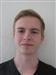
\includegraphics{pictures/s123161.png}%

\includegraphics{pictures/s123369.png}%
\end{figure}
22nd of May 2013

\thispagestyle{empty}
\newpage

 


%TODO abstract
%TODO resum�
%TODO whodunnit
\clearpage
\tableofcontents
%TODO problemdecription
%specifications
\section{Specification}
We have chosen to make an arkanoid like game with the following extensions

\begin{enumerate}
\item Continuously calculated reflection angle from the striker.
\item Bricks with any number of lives, colored after this number.
\item Background music.
\item Sound effects.
\item ASCII art backgrounds generated from real pictures.
\item Analog joystick input.
\item A score system.
\item Multiple levels.
\item Limited number of player lives.
\item 30 frames per second graphics.
\item Powerups.
\item Highscores saveable on permanent media.
\end{enumerate}

The list is ordered with items in descending priority. The last 2 items on the list
did not make it into the final game due to time constraints.

%overall analysis
\section{Analysis}
As the game must be made to run on an eZ8 microcontroller, with limited performance capabilities, and display graphics in a terminal
 via ANSI commands sent over a relatively low bandwidth UART connection, performance must be taken into consideration and bottlenecks identified. \\

Generating the sound needed for background music and sound effects is a performance heavy task that we deemed
impossible to implement purely on the eZ8 microcontroller.
Therefore, the sound generation is offloaded to a Stellaris Launchpad microcontroller. 
This will then recieve commands from the eZ8 using SPI, such that the game running on the eZ8 can control
what sounds are being generated by the stellaris.\\

Displaying background images requires a lot of ANSI escape codes to be sent over the UART communication with
the terminal used for graphics. This is due to complex graphics having many different colors. As the UART on the eZ8 
development board is only capable of sending data at 115200Baud, this issue must be taken into account
in the software responsible for graphics if a new picture is to be rendered 30 times a second. \\

To make use of a joystick for controlling the striker it will also be necessary to use the ADC on the eZ8 development
board. 






%design top
\section{Design}
This section covers both game design and software architecture design, as well as the
design of the individual software modules.

\subsection{Game Design}
The game is an arkanoid clone and as such it is very simple and follows the general arkanoid formula of destroying
bricks using a ball that bounces around the screen. The ball will reflect itself off of a brick, wall
in the top of the playing space as well as two walls bordering the sides of the playing space.
There is nothing stopping at the bottom of the playing space, except the player controlled striker.
It is the players objective to control the striker such that the ball is reflected off of it and
hits all the bricks. Thereby destroying the bricks. \\

In this version of arkanoid, which we will henceforth refer to as Smashing Bricks, the player
upon starting a game is presented with a splash screen, followed by the first level. The levels
themselves contain a brick layout that can be changed as well as a monochrome background image.
Upon completion of the level, the full-color background image is revealed and the player can
move on to the next level. Once the player reaches the end of the game, the players score
will be presented and the option to restart the game will be available. \\

The score is incremented by a set amount every time a brick is hit or destroyed. If the player
misses the ball, another amount is subtracted from the score. If the players score goes below
0, the game is over and the player will have the option to restart the game. \\

The balls reflection from the striker is not actually a reflection, instead the direction
of the ball is changed according to where it hit the striker. As with all games, these
mechanics are based on their feeling and this to us felt like the most natural way to play.
Similarly the speed of the ball and striker are also based on feel. \\

Background music will play and sound effects are triggered every time the ball is reflected
from a brick, a wall or the striker. \\

The game only has a single difficulty, hard, this is due to the fact that we deemed slow and/or
easy arkanoid games to get boring too quickly. The game is therefore deliberately designed to 
force the player to quickly be able to estimate where the ball will reach the bottom again, as 
soon as it leaves the striker.

\subsection{Software Architecture Design}
Considerable time and effort went into insuring that the software itself would be modular and easily extensible.
As mandated, the software contains three layers. A hardware layer that is concerned only with
direct hardware manipulations, an API layer that is concerned with presenting general functionality to
the final application layer. The layers can be changed individually as long as they present the
same functionality to the layer directly above. \\

In our design, the hardware layer is relatively small as it only needs to deal with the following:

\begin{itemize}
	\item Handle ADC input for the joystick.
	\item Set up timers.
	\item Send data over SPI.
\end{itemize}

It is not necessary to write software that controls the UART as API functions covering  this
 is already provided by the default eZ8 libraries included in ZDS. \\

The API functions needed for general game applications are then the following.

\begin{itemize}
	\item Graphics.
	\item Sound.
	\item Math. (Sine, Cosine, fix point etc.)
	\item Input handling.
\end{itemize}

The API layer presents a general framework that can be used for any game application. If extra
functionality is needed it is also easily extensible. \\

To make the game application itself as modular and extensible as possible, we have utilized a
style of C programming that approaches object oriented programming as this is especially well
suited for games. To understand why, we must look at the general game application control flow. \\

Modern games run either with a fixed or a free running framerate, we will only discuss the fixed
framerate type as this is easier to work with for this application. Within every frame period, the
game situation is updated. This means getting input from the user and  updating the position of every object
, checking collisions and reacting accordingly etc. When this is done, the new situation is presented to the
 user by updating the graphics medium, in this case a terminal. The cycle then repeats until the game
ends. This can be split into 3 distinct operations that need to be performed within the main game loop:
Get input, update, render. This will be done at the standard 30 frames per second \\

The advantage of object oriented programming is that all game entities can then contain their own
update and render functions, eliminating the need to change exisiting code when a new game entity is added.
This also helps to avoid spaghetti code and deep nesting problems. While we are aware that object oriented
programming usually comes with significant performance overhead and as such is not suitable for a microprocessor,
we deem this to not be a problem as we do not a use truly object oriented style, only an approximate one, where every
entity is represented as a struct with function pointers to its inner "methods" and primitives for fields.
Only a small amount of glue code is needed to control the transition between levels and manage the game state. \\

Communication between modules follows the mantra that less is good. As such, the amount of information and functions
present to each other is kept at a minimum. This is done to keep the number of entry points to a module as small
as possible, thus making it possible to change the inner workings of a module without breaking external dependencies.
As functions and variables in C are confined to their own scope, the file in which they are declared, and this
scope can only be extended by including them in a header file, our header files are kept as simple as possible. \\

A block diagram of the modules and their communication paths can be seen in figure \ref{architecture_block}. In the
diagram, arrows represent in which direction function calls and commands travel, which typically means information
flows in the opposite direction. \\

\begin{figure}
	\center
	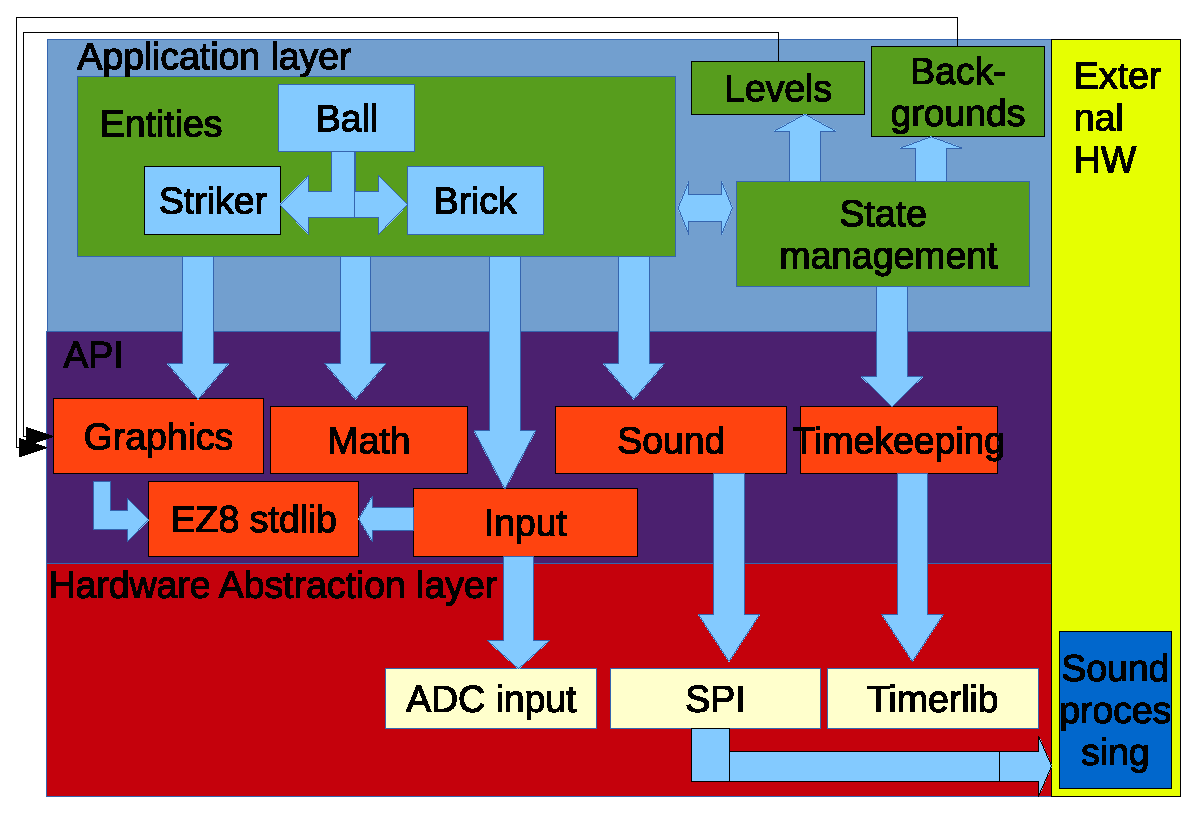
\includegraphics[scale=0.7]{pictures/architecture_block.eps}
	\caption{Block diagram of the software modules and their communication}
	\label{architecture_block}
\end{figure}

A flowchart depicting the top level control flow can be seen in figure \ref{top_flow}.

\begin{figure}
	\center
	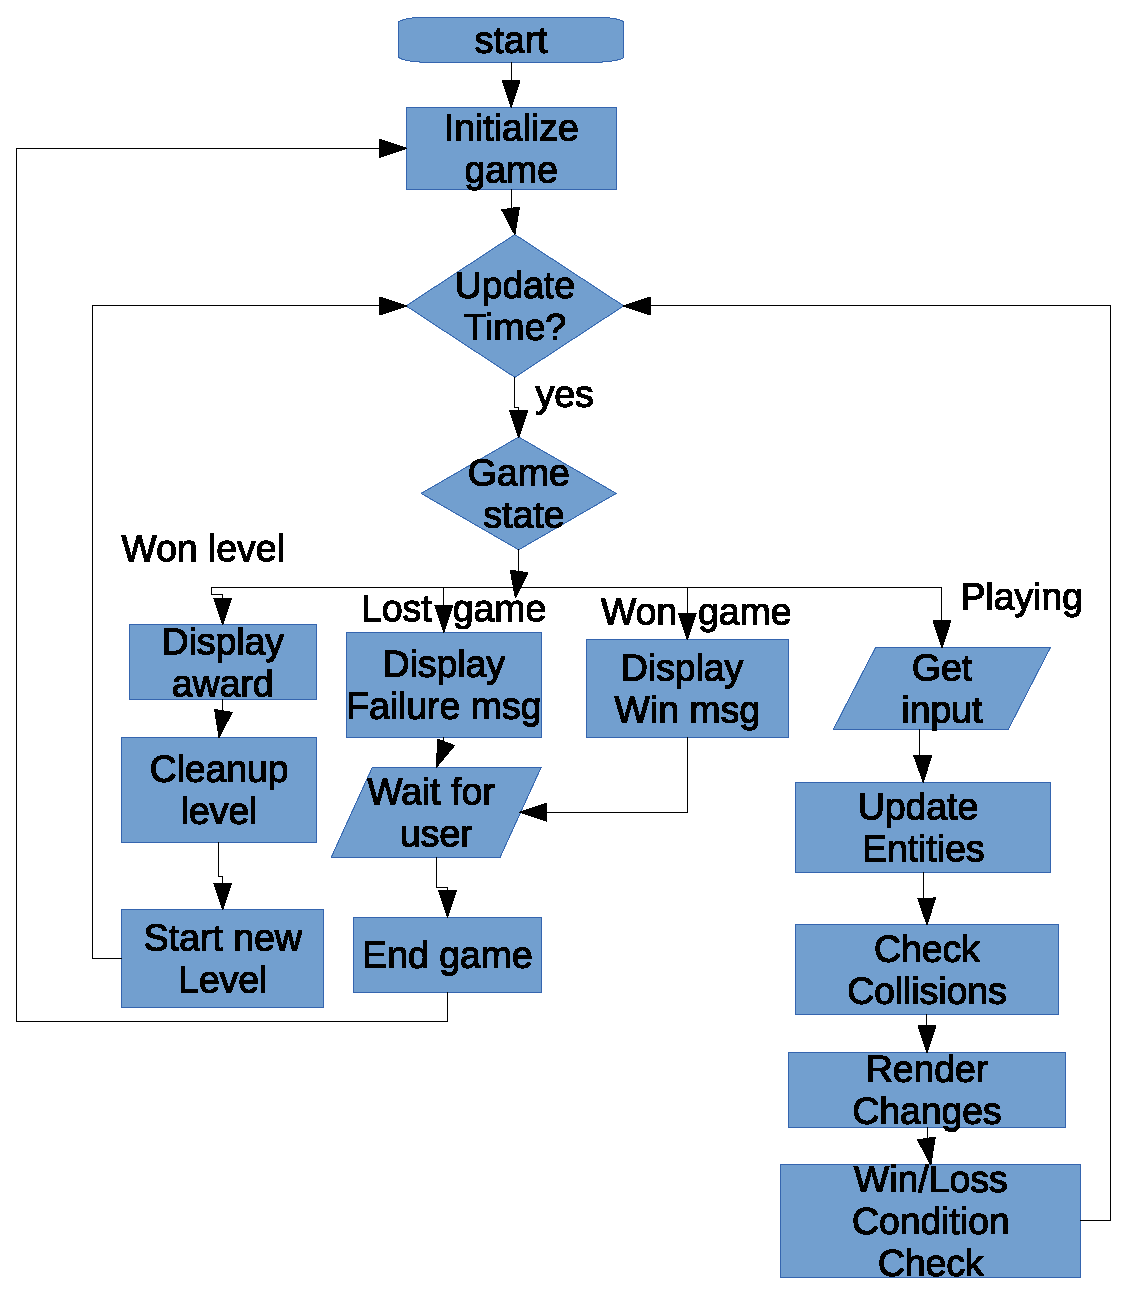
\includegraphics[scale=0.7]{pictures/top_flow.eps}
	\caption{Control flow at the top level}
	\label{top_flow}
\end{figure}


%%TODO Gaming units

	%TODO analysis 
	%TODO desing
	%TODO implementation
	%TODO result

%TODO %Audio unit
	\subsection{Audio module introduction}
The audio module will be run as an external application on a \emph{Texas
Instruments} \emph{Stellaris Launchpad}, communicating with the \emph{eZ8} via
\emph{SPI}.

The audio module performs the following:
\begin{itemize}
  \item Play and stop one song: \emph{Popcorn}
  \item The song has 3 voices
  \begin{itemize}
    \item Lead
    \item Bass
    \item Percussion
  \end{itemize}
  \item The module connects to the \emph{eZ8} with SPI and receives data as
  \emph{MIDI} messages.
  \item The module can play game specific sounds (bleeps when the ball hits
  anything and similar)
\end{itemize}

Since this section assumes some known knowledge about synthesizers, a small
introduction to subtractive synthesis is given in the next section.

\subsubsection{An introduction to subtractive synthesis}\label{synthxp}
Subtractive synthesis is one of the very popular methods of creating musical
notes. A very basic synthesizer is described in figure:~\ref{fig:basicsynth}

\stdfig{0.8}{audiomodule/basicsynth}{Block diagram of a basic
subtractive synthesizer, with examples of signal waveforms. A
sequencer is used as the source of notes. Note that the timing
of the sequencer signal examples is not one scale with the
rest of the signal examples.}{fig:basicsynth}

A steady stream of pulses enters the sequence and makes it advance through it's
pattern, here with a pattern length of 5. The sequencer output is used as the
input of the oscillator to control the frequency of it - this could just as well
be from a keyboard - The oscillator generates a harmonic rich output that is fed
into a resonant filter (2 pole low-pass here) to \emph{subtract} harmonics; then
the filtered signal is fed through an amplifier.

The cutoff frequency of the filter is controlled by the \emph{ADSR}, an acronym
for \emph{Attack Decay Sustain Release} this works as following:
\begin{itemize}
  \item Attack: After a trigger the output rises from 0
to max at a specified rate.
  \item Decay: The signal then falls to the sustain level at a specified rate.
  \item Sustain: As long ad the gate is high, the output is helt at the sustain
  level.
  \item Release: Once the gate is low, the output falls back to 0 at a specified
  rate.
\end{itemize}

The amplitude of the amplifier is controlled by an \emph{AHDSR}, the same as the
\emph{ADSR}, except a short delay, where the output is held at max - the hold
phase - is put in between the attack and decay stages.
 
	%analysis 
	\subsection{Audio module analysis}
The audio generation is very processor heavy - if more than monophonic
bleeps are desired that is. - To produce alias free audio in the full audible
range, the output has to be updated more than 40000 times a second.
Therefore this task is moved from the \emph{eZ8} to a \emph{Texas
Instruments} \emph{Stellaris Launchpad}, an evaluation-board for the 80MHz
\emph{ARM Cortex-4M} \emph{LM4F120H5QR} chip.
%TODO tilf�j link til http://www.ti.com/tool/EK-LM4F120XL

The \emph{LM4F120H5QR} is ideal as:
\begin{itemize}
  \item It has 64kB of FLASH memory, enough for a medium-size program and small
  wave-files;
  \item 32 bit processor, providing a solid frame for fast and
  precise generative sound synthesis;
  \item build in PWM module that width some external filtering can be used a a
  digital to analog converter, removing the need for an external ADC. Furthermore
  the output is powerful enough to drive small headphones at low volumes.
  \item We have past experience with the processor and associated tools, thus
  the time cost can be reduced by choosing this solution over another.
  
\end{itemize}

As the audio module has to play both a piece of music and sound-effects; a mix
of generated sounds and playback of wave-files is chosen.

The use of generated music cuts down the space a huge wave-file would take. 10s
of 8bit data at 44kHz is 0.44MB, we can't fit that in the 64kB FLASH of the
\emph{LM4F120}. On the other hand even at 80MHz speech synthesis becomes
troublesome, but if speech is re-sampled to ~10kHz it is still possible to make
out words. Percussion sounds can also be put in down-sampled wave-files, as
aliasing artifacts aren't a huge sacrifice when dealing with short, rhythmic
outbursts.



	%TODO desing
	\subsection{Audio module design}

As described under the analysis, the audio module has to be capable of both
generating sounds and playing predefined wave-files. The processor is chosen to
run in real-time with a frequency of 44kHz, this is done to reduce aliasing
artifacts - in theory this is enough to allow an output spanning the full
audible range, given sufficient filtering and taking care not to generating any
tones above the nyquist-frequency; we did however not have the time to dive
fully into this theory and thus some aliasing will occur.

The design of the audio module will be done like a digital model of a modular
synthesizer, taking inspiration from eg. the free-to-try software
\emph{SynthEdit0} in which different block (oscillators, filters, transient
generators, wave-file players etc.) can be connected to form whole synthesizers.
See figure:~\ref{fig:synthedit}.

\stdfig{0.8}{audiomodule/synthedit.jpg}{The design of the synthesizers took
inspiration from the block approach as seen in eg. the free program
\emph{Synth Edit} \cite{SynthEdit}. Image from \cite{SEimg}}{fig:synthedit}

This approach allows for both easy programming of the modules, as this becomes
an highly manageable problem; easy programming of the synthesizers, this is just
connecting the blocks; and provides an easily expandable and reusable library.
This also allows for easy programming reusable container modules, eg. a
standard synthesizer.

Communication is done over SPI, using MIDI (\emph{Musical Instrument Digital
Interface}) commands. This allows for a MIDI interpreter module, working in
similar ways as all other modules.

\subsubsection{Overview}
We decided that the background music should be the 80'es classic
\emph{Popcorn}.
For this we need three voices, lead, bass and percussion.
The score is stored in 6 arrays (notes and gate/trigger for each voice) and a
sequencer goes through this array, giving notes and triggers to the synthesisers
and wave-player. This is illustrated in figure:~\ref{fig:audioflow}

\stdfig{0.8}{audiomodule/audioflow}{Block diagram of the audio
module}{fig:audioflow}

The two red blocks, \emph{raw Synth} and \emph{filter Synth} are the
synthesisers for the lead voice and the bass voice respectively. These modules
are application specific.

For the lead voice we create a module called `\emph{RawSynth}, because this only
contains the bare minimums for a synth: An oscillator with a wave-shaper and a
\emph{AHDSR} module, controlling the volume. The wave shape is set to a stepped
saw-wave. See figure:~\ref{fig:rawsynth} for a block diagram.

\stdfig{0.8}{audiomodule/rawsynth}{Block diagram of the RawSynth used for the
lead voice}{fig:rawsynth}

For the bass voice we choose a synth with a 2-pole resonant state variable
filter, using the low-pass, doing a downward sweep for a synthy \emph{``dauww''}
sound. a block diagram for this can be seen in figure:~\ref{fig:filtersynth}.
This module we name \emph{FilterSynth}, a square wave is chosen for the
wave table, as this gives a nice tone for the bass (the fundamental is strong
in a square wave, compared to eg. saw wave)

\stdfig{0.8}{audiomodule/filtersynth}{Block diagram of the FilterSynth used for
the bass voice}{fig:filtersynth}

\subsubsection{Design of the core modules}
The following core modules were designed:
\begin{itemize}
  \item VCO: A basic oscillator with an input for the note to play and a saw
  wave output, no bandwidth limiting.
  \item LFO: A basic low frequency oscillator with a saw wave output and a
  \emph{tick} output, a delta function once every cycle.
  \item Sequencer: A sequencer, takes an array and turns it into a sequence -
  outputting each element in the array one at a time. The sequencer advances
  when the tick input is high and resets when the reset is high. The sequencer
  also has an output producing a delta function when looping around.
  \item LowPass: A simple 1-pole \emph{IIR} low-pass filter. Has an input for
  the signal and filter coefficient. This module was not used in the final product.
  \item SVF: A 2-pole resonant state variable filter. Has inputs for signal,
  filter coefficient, damping coefficient and outputs for hi-pass, band-pass and
  low-pass.
  \item AHDSR: \emph{Attack Hold Decay Sustain Release} module as described in
  section \ref{synthxp}. Has inputs for trigger, gate and the 5 parameters. only
  has one output.
  \item WaveShaper: A module capable of turning a saw wave from the VCO into any
  wave-shape - provided this wave-shape is given in an array. Can also perform
  bandwidth-limited wave-shaping if the supplied array supports it.
  \item MidiInterpreter: A module capable of reading from a FIFO (\emph{First
  In First Out}, as opposed to a stack) buffer and interpreting these signals.
  Has outputs for note: the last note played; trigger: high if the note was
  played in the current frame and playing: indicating if the music should be
  playing or not. Ideally there would be a ``note on'' and ``trigger'' array for
  every note (127 notes) on every midi channel (8 channels) - but this was not
  optimal for the given processor.
  \item OneShotter: A module for playing back small wave-files. It can
  re-trigger and takes a pointer to an array, storing the wave-file and the
  length of said file as arguments when updating.
\end{itemize}

\subsubsection{Design of the FIFO buffer}
A general utility structure \emph{FIFOBuffer} is designed, this module has the
following functions:
\begin{itemize}
  \item push: Pushes a data point into the beginning of the FIFO, returns 1 on
  success and 0 if the buffer is full.
  \item peak: Get the value of a data point a specified length from the end of
  the FIFO. Returns 0 if no data point exists here and 1 if it does.
  \item pop: Pop a data element from the end of the FIFO. Returns 1 if there
  was an element to pop and 0 if the FIFO is empty.
\end{itemize}

	%TODO implementation
	\subsection{Audio module implementation}

The structure of the program deviates a bit from the three layers described in
\cite{Lect2} on slide 9, there is no application interface layer - as seen in
figure:~\ref{fig:overview}

\stdfig{0.8}{audiomodule/overview}{Block diagram of overall program
structure}{fig:overview}

The two main reasons for this is:
\begin{itemize}
  \item There are very few functions in this layer - a
layer more would just be a pass-through layer.
  \item For testing the application had to be ported to \emph{Windows}
\end{itemize}
	%TODO result (wave files)
	
%%TODO Display unit (PuTTy)
	
	%TODO analysis

%result?
%tests?
%conclution

%litterature
\bibliographystyle{IEEEannot} %eller et andet setup?
\bibliography{audio_module/litt}
% build from cmd with 
%"C:\Program Files\pgm\MiKTeX 2.9\miktex\bin\x64\bibtex.exe" -include-directory="C:\Users\Soren\Git\30010\rapport\rapport" -include-directory="C:\Users\Soren\Git\30010\rapport\rapport\tmp" "C:\Users\Soren\Git\30010\rapport\rapport\tmp\main.aux"

%appendix
%TODO journal






\end{document}


